The software architecture may be of interest to developers of tree editors and similar kinds of \gls{VSCode} extensions.
There is potential to directly reuse components from this design.

\subsection{Architecturally Significant Requirements}
The high level software architecture for the tree editor was shaped mainly by three \acrfullpl{ASR}.
The editor must be a \gls{VSCode} extension, the tree viewer must use the \gls{VSCode} Custom Editor \gls{API}, and the extension must reuse \acrshort{EMF} java code and the EMF.Cloud Model Server.
This results in a system of three main components: a \textit{Tree editor frontend}, a \textit{Tree editor extension} and a \textit{Tree Language Server}.

Another \acrshort{ASR} is that the model may change, and the rest of the system must respond and be updated.
Therefore, a bi-directional communication between components is established, and an event driven architecture is used.
The communication is isolated and standardized in a protocol, called the \textit{Tree Language Server Protocol} (\acrshort{TLSP}).
This protocol is presented in detail in \cref{sec:tlsp}.


\subsection{Changes from pre-project}
From the pre-project, the high level architecture (see \cref{fig:pre-project-tree-editor-architecture}) changed mainly by avoiding the EMF.Cloud Model Server as a separate running process, and is now embedded inside the Tree Language Server~\cite[p.~49]{rekstadModelingEnvironmentCloud2020}.\\

On the code level, only the extension code and tree document model are similar.
The tree document model has changed to accommodate multiple roots, by introducing the \textit{TreeRoot} and moving the \textit{ArchitectureSchema} and \textit{IconConfiguration} as children of these root, instead of the \textit{TreeDocument}.
This allows configurations to be different on a per-root basis, which is needed when for example opening both a GenModel and \gls{Ecore} model in the same document.\\

The frontend is different from the pre-project prototype by using the \textit{Vue.js} framework, and implementing actual features.
The pre-project was only an example viewer, not communicating with the extension.\\

For the EMF.Cloud Model Server, this is now bundled inside the Tree Language Server, instead of a separate component.
The pre-project used \gls{REST} to communicate, while now it happens in java by using the classes of the EMF.Cloud Model Server, then relaying the answers over \acrshort{TLSP}.
The pre-project did not implement any real logic inside the server either.


\subsection{System explanation}
This section will explain the software architecture through a series of diagrams called the \textit{C4 Model} (Context, Container, Component, Code)~\cite{simonbrownC4ModelVisualising}.
This is a top-down approach where one ``zooms'' in on the system components, so the wider context is clear.


\subsubsection{Context}
At a high level, the system has students interacting with \gls{Gitpod}.
The developed system runs inside \gls{Gitpod} as an extension.
This is illustrated in \cref{fig:gitpod-system-context}.
The student use \gls{Gitpod} as a development environment, where they use the \acrshort{IDE}, change files in a Workspace, and runs programs in a terminal.
\Gls{Gitpod} uses \gls{git} to retrieve the student's code from \gls{GitHub}, and pushes changes back to it.

When a Student wants to install an extension to the \acrshort{IDE} in \gls{Gitpod}, it can either let the Student upload an extension file, or search the publicly available extensions in the OpenVSX extension registry.
The instantiated artifact from this thesis could be uploaded to OpenVSX.


\begin{figure}[H]  % order of priority: h here, t top, b bottom, p page
  \centering
  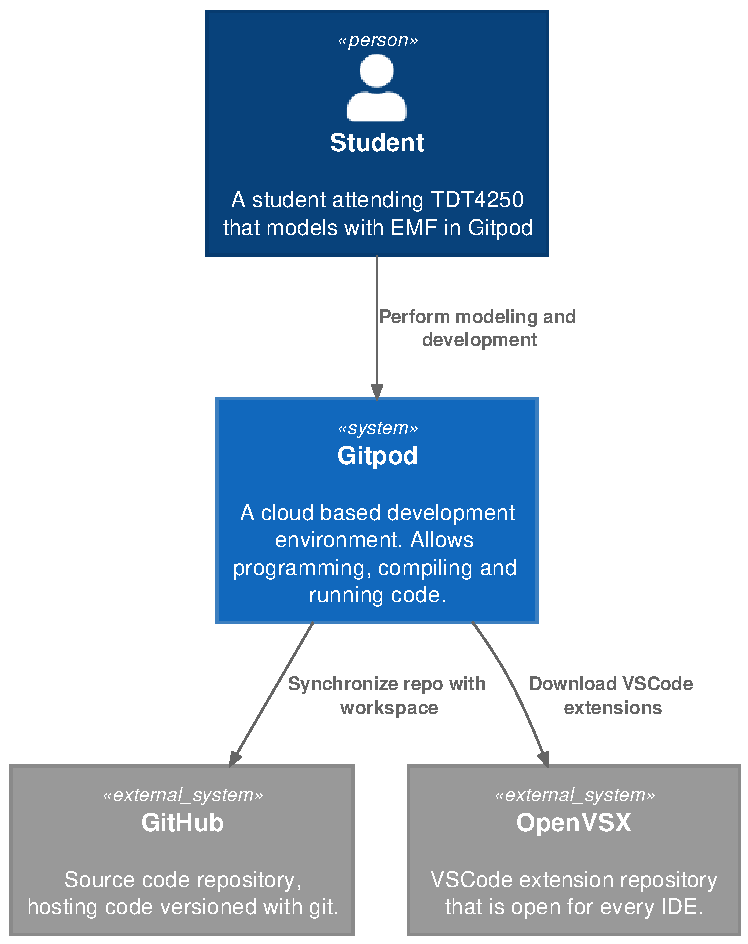
\includegraphics[width=\textwidth]{figures/plantuml/Gitpod_context.pdf}
  \caption[System context diagram for Gitpod]{A system context diagram for Gitpod. The extension will run inside the Gitpod service, used by a student to do modeling and developing. Gitpod uses git to synchronize code with GitHub. The extensions in Gitpod are downloaded from a service called OpenVSX.}\label{fig:gitpod-system-context}
\end{figure}

\subsubsection{Containers}

Inside the \gls{Gitpod} system, there is a \acrshort{IDE}, the \textit{Ecore Tree Editor Extension} from this thesis, and the Workspace.
This is shown in \cref{fig:gitpod-container-diagram}.
The \acrshort{IDE} can be \gls{Theia} or \gls{VSCode}.
This \acrshort{IDE} is responsible for providing the user interface to the student.
It also has the responsibility of installing and activating the extension.
The extension runs in the environment provided by the Workspace.
For example, the operating system and the available programs are provided by the Workspace, as well as the student's project files.
If the extension wants to run a java program, the Workspace must have a Java Runtime installed.

\begin{figure}[H]  % order of priority: h here, t top, b bottom, p page
  \centering
  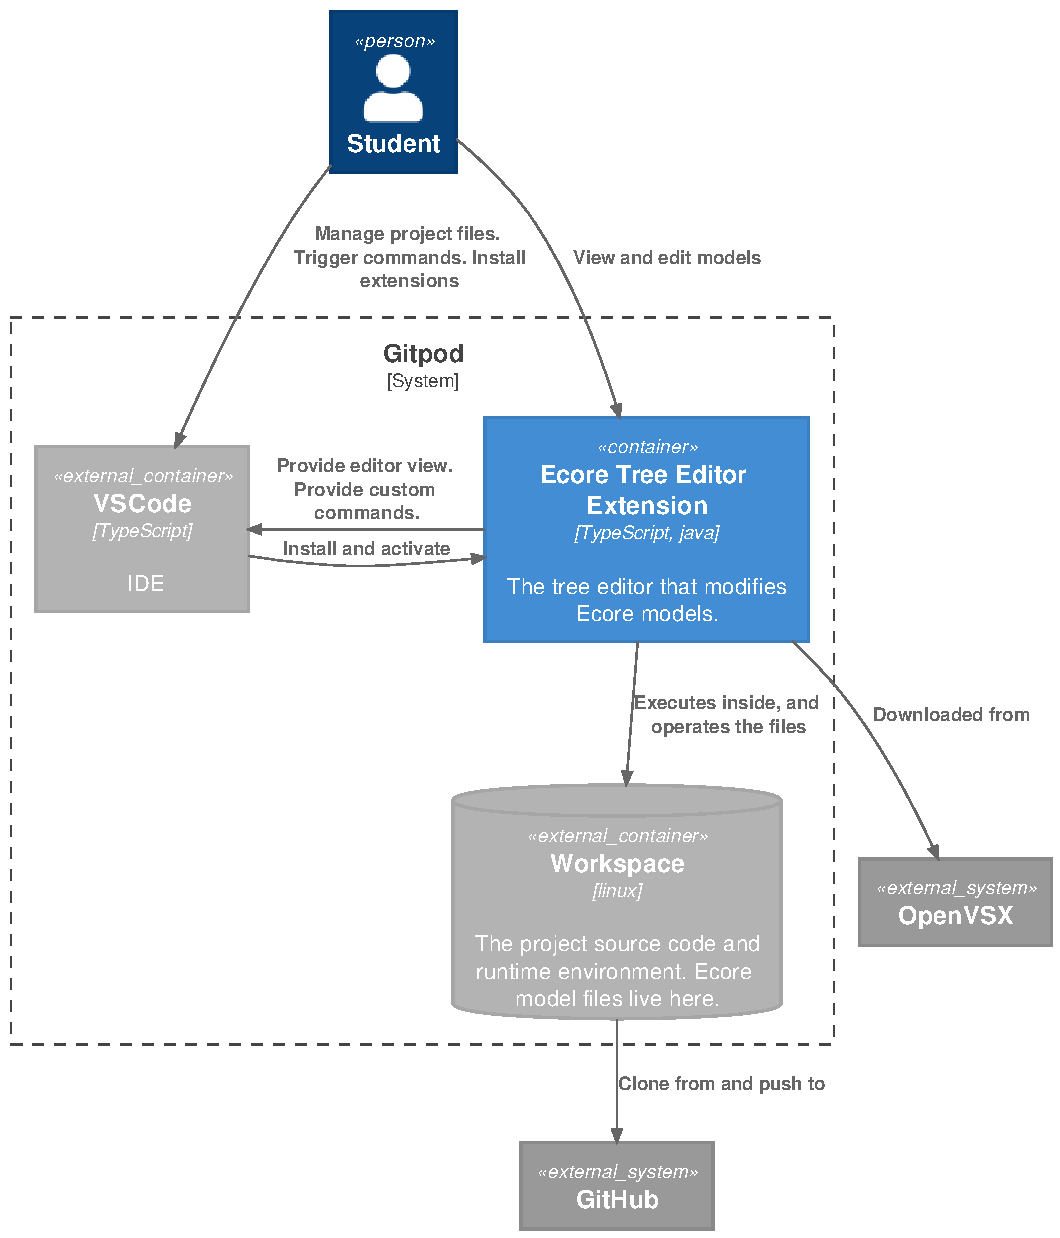
\includegraphics[width=\textwidth,height=\textheight,keepaspectratio]{figures/plantuml/Tree_Editor_Extension_container.pdf}
  \caption[Gitpod container diagram]{Container diagram for gitpod. The Gitpod system from \cref{fig:gitpod-system-context} is expanded to show its internal components. The \acrshort{IDE} used by Gitpod is \gls{VSCode}.
  The student will interact with VSCode, and install the Ecore Tree Editor Extension created from this thesis.
  This extension will also provide a user interface, which the student uses for modeling.
  This extension reads files from the Gitpod workspace, and uses the runtime provided by the workspace such as a Java Runtime Environment.}\label{fig:gitpod-container-diagram}
\end{figure}


\subsubsection{Components}

The Ecore Tree Editor Extension itself consists of three main components.
It is the \textit{Tree editor extension} (or simply ``extension''), which integrates with \gls{VSCode} or \gls{Theia}.
Then there is the \textit{Tree editor frontend} (or ``frontend''), which provides a user interface with the hierarchical tree structure, labels and icons to the student.
The last component is the \textit{Tree Language Server} (TLS, or ``server''), a java based server with knowledge about \acrshort{EMF} and the EMF.Cloud Model Server.
This is shown in a deployment diagram in \cref{fig:gitpod-deployment-diagram}.\\


\begin{figure}[H]  % order of priority: h here, t top, b bottom, p page
  \centering
  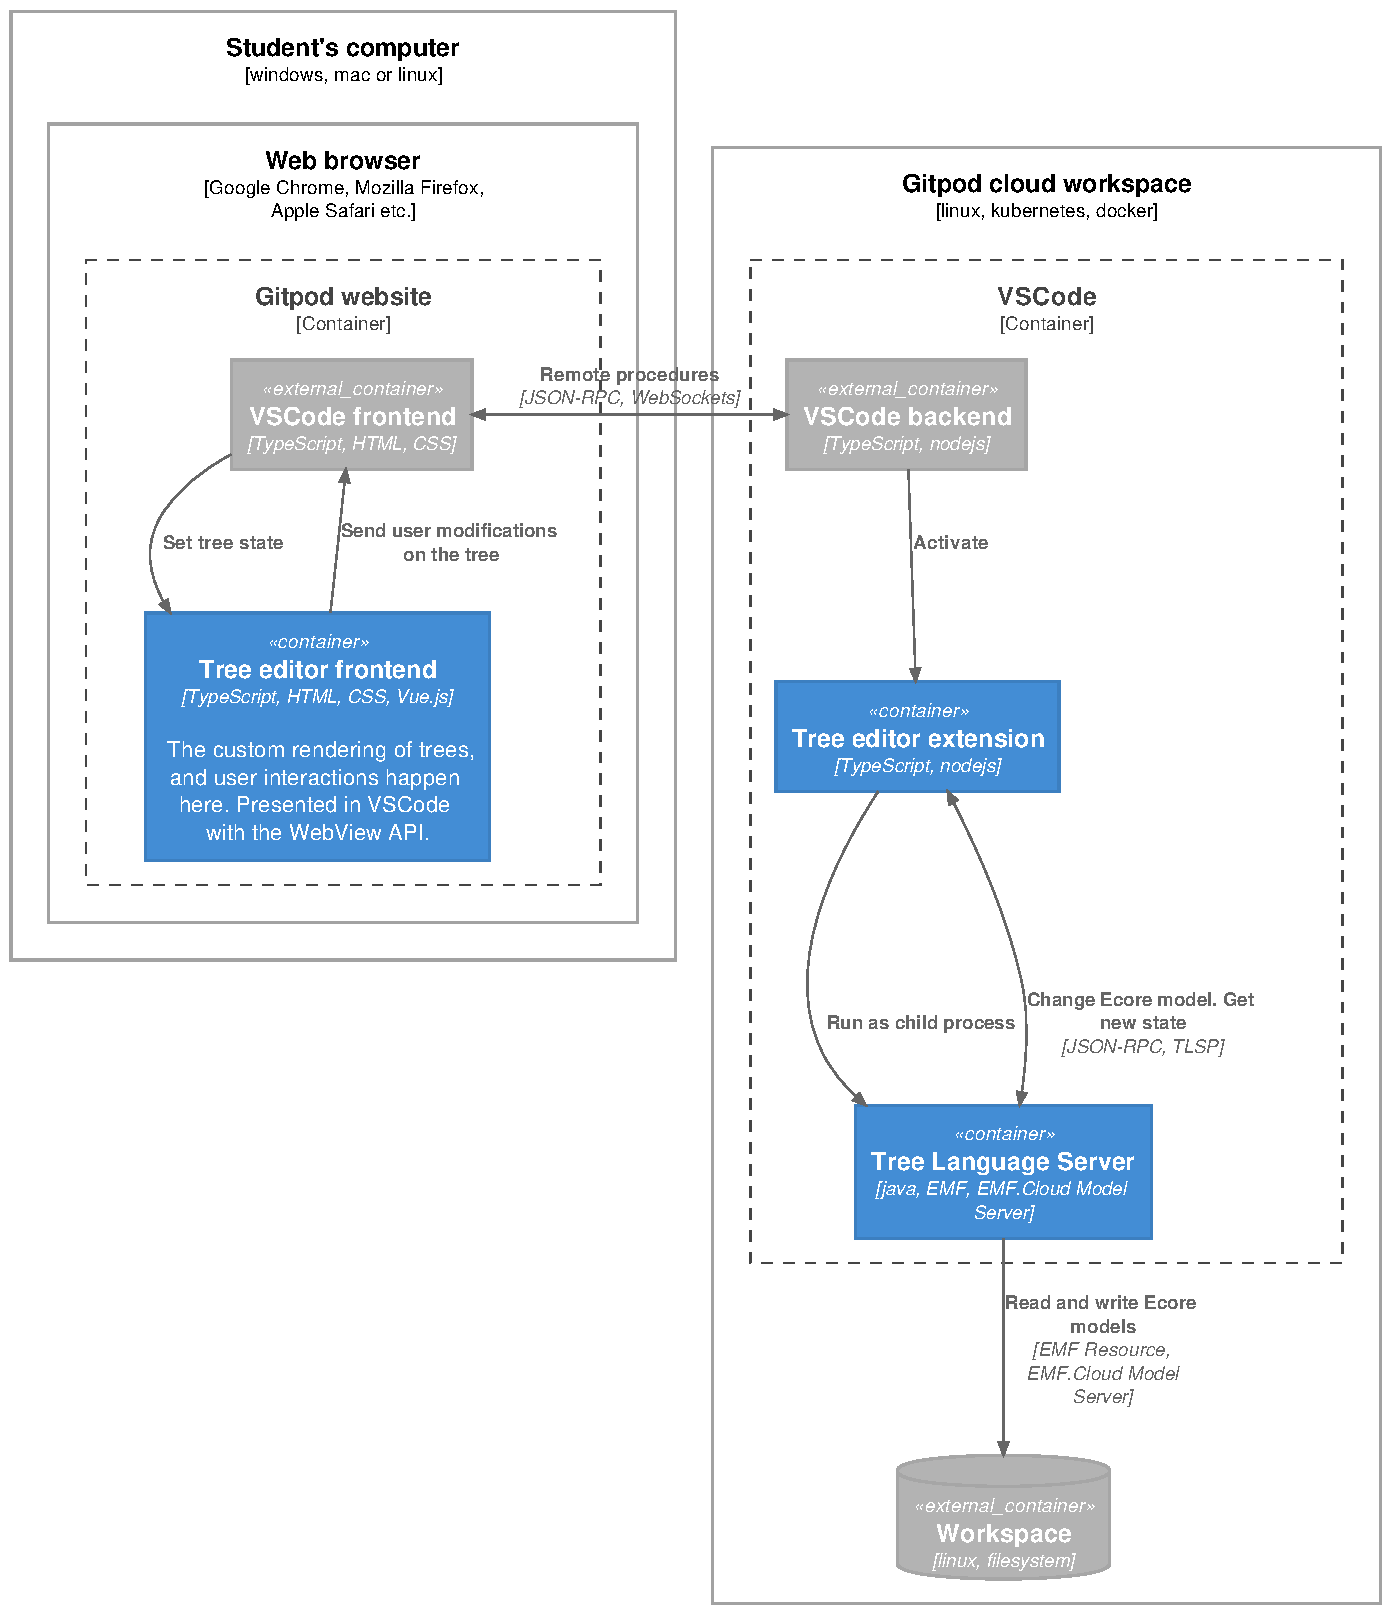
\includegraphics[width=\textwidth,height=\textheight,keepaspectratio]{figures/plantuml/Tree_Editor_Extension_deployment.pdf}
  \caption[Gitpod deployment diagram]{Deployment diagram of Gitpod. The student will use their computer to load the Gitpod website.
  The Gitpod service will start a computer in a cloud provider, to create a cloud workspace.
  The student only loads the VSCode frontend and Tree editor frontend into their browser.
  VSCode has a backend which runs inside the Workspace, and communicates to the frontend over WebSockets, using JSON-RPC\@.
  The VSCode backend will activate the Tree editor extension, which in turn will start a Tree Language Server.
  This Tree Language Server runs java, and reuses the \acrshort{EMF} tooling.
  The Tree editor extension communicates to the Tree Language Server over a well defined protocol, where it asks to read model files, and execute commands to change the models.
  The Tree Language Server uses the Workspace to read and write \texttt{.ecore} files.}\label{fig:gitpod-deployment-diagram}
\end{figure}

The Tree editor extension and Tree Language Server talk together using a protocol named \acrfull{TLSP}.
This protocol is another design artifact from this thesis, and is described later in \cref{sec:tlsp}.
This protocol knows nothing about \acrshort{EMF}, and the same with the Tree editor frontend.
These two parts of the design only work on generic tree structures, as described in \cref{sec:tree-structures}.\\

The Tree editor extension is the component responsible for providing both the Tree editor frontend, and the Tree Language Server.
It also knows about \acrshort{EMF}, because it registers the \texttt{ecore}, \texttt{genmodel} and \texttt{xmi} file extensions to \gls{VSCode} and \gls{Theia}.
The custom Commands from the \acrshort{IDE}'s Command Palette are provided by this Tree editor extension as well.\\

Any changes to the student's model files are saved to disk by the Tree Language Server.
The Tree editor frontend is close to stateless, and the Tree editor extension only bridges the Tree editor frontend and the TLS.

\subsubsection{Code}

\paragraph{Modules}
At a code module level, the Ecore Tree Editor extension is made of 5 modules.
The extension, frontend, server, and two shared libraries: \textit{Tree Document model} and \textit{VSCode and Webview RPC} (or simply RPC library).
The frontend and extension both use the Tree Document model and the RPC library.
This is shown in \cref{fig:extension-code-modules}.
All the modules are coded with \gls{TypeScript}, except the server, which uses Java.\\

The server also ``uses'' the Tree Document model, but by re-implementing\footnote{Not ideal, but no good transpiling (programming language translating) software was found in a reasonable amount of time, to automate this.} it in java.
The Tree Document model module is the result of using Domain Driven Design and a layered architecture (by \textcite{evansDomaindrivenDesignTackling2004}).
It encapsulates the concepts and business logic related to editing tree structures.


\begin{figure}[htbp]  % order of priority: h here, t top, b bottom, p page
  \centering
  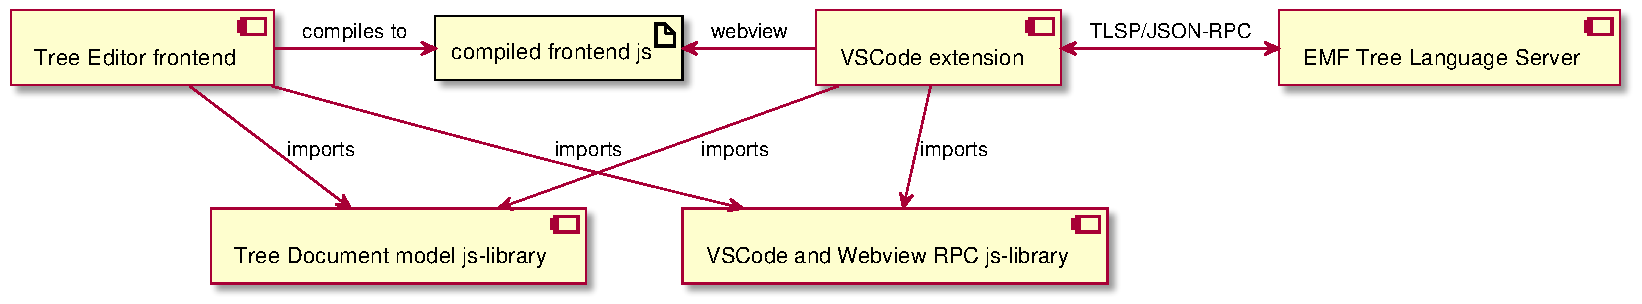
\includegraphics[width=\textwidth]{figures/plantuml/Tree_editor_components.pdf}
  \caption[Ecore Tree Editor component diagram]{Component diagram of the Ecore Tree Editor.
  The for the the extension is organized in 5 separate modules.
  The main module is the VSCode extension.
  This extension bundles the compiled frontend javascript artifact, and the compiled EMF Tree Language Server java jar-file.
  The Tree DOcument model js-library is the layer with the domain model for tree editors.
  It is used in both the frontend and the extension.
  }\label{fig:extension-code-modules}
\end{figure}

\paragraph{Classes}
Three \gls{UML} class diagrams are presented, one each for the frontend, extension and server.
These are not complete, meaning some classes, properties, methods and relationships are not shown.
This is intentional, to increase the clarity, comprehension and the essence of the diagrams.

\paragraph{Frontend classes}
A diagram of the frontend is shown in \cref{fig:tree-editor-frontend-code}.
The execution environment for this is a web browser frame, meaning it has access to the HTML DOM\footnote{Document Object Model, which is how a web browser represents web pages.}.
It has a view layer using a framework called \textit{Vue.js}.
The frontend's state (\texttt{TreeDocument}) is held in a state storage called ``Store'', using a library called \textit{Vuex}.
This state can only be changed through explicit mutations and actions.
This is so the store can intercept changes, and send them to the server via the extension, over the \acrlong{TLSP}.
The frontend talks to the extension using a \texttt{VSCode} interface, where the actual \gls{VSCode} \acrshort{IDE} injects an implementation.
A mocked version (\texttt{MockVSCode}) is provided as an implementation when testing and developing the frontend outside of the \gls{VSCode} \acrshort{IDE}.
Two classes help the communication between the extension and frontend: \texttt{TreeEditorWebview} and \texttt{VscodeExtension}.
These utilize a \gls{JSON-RPC}-like protocol, over the \texttt{VSCode} method called \texttt{postMessage} and the javascript \texttt{Window}'s \texttt{addEventListener}.
The \texttt{FormEditor} view is intended to use the JSON-Forms library, but this view is not finished.

\begin{sidewaysfigure}[htbp]  % order of priority: h here, t top, b bottom, p page
  \centering
  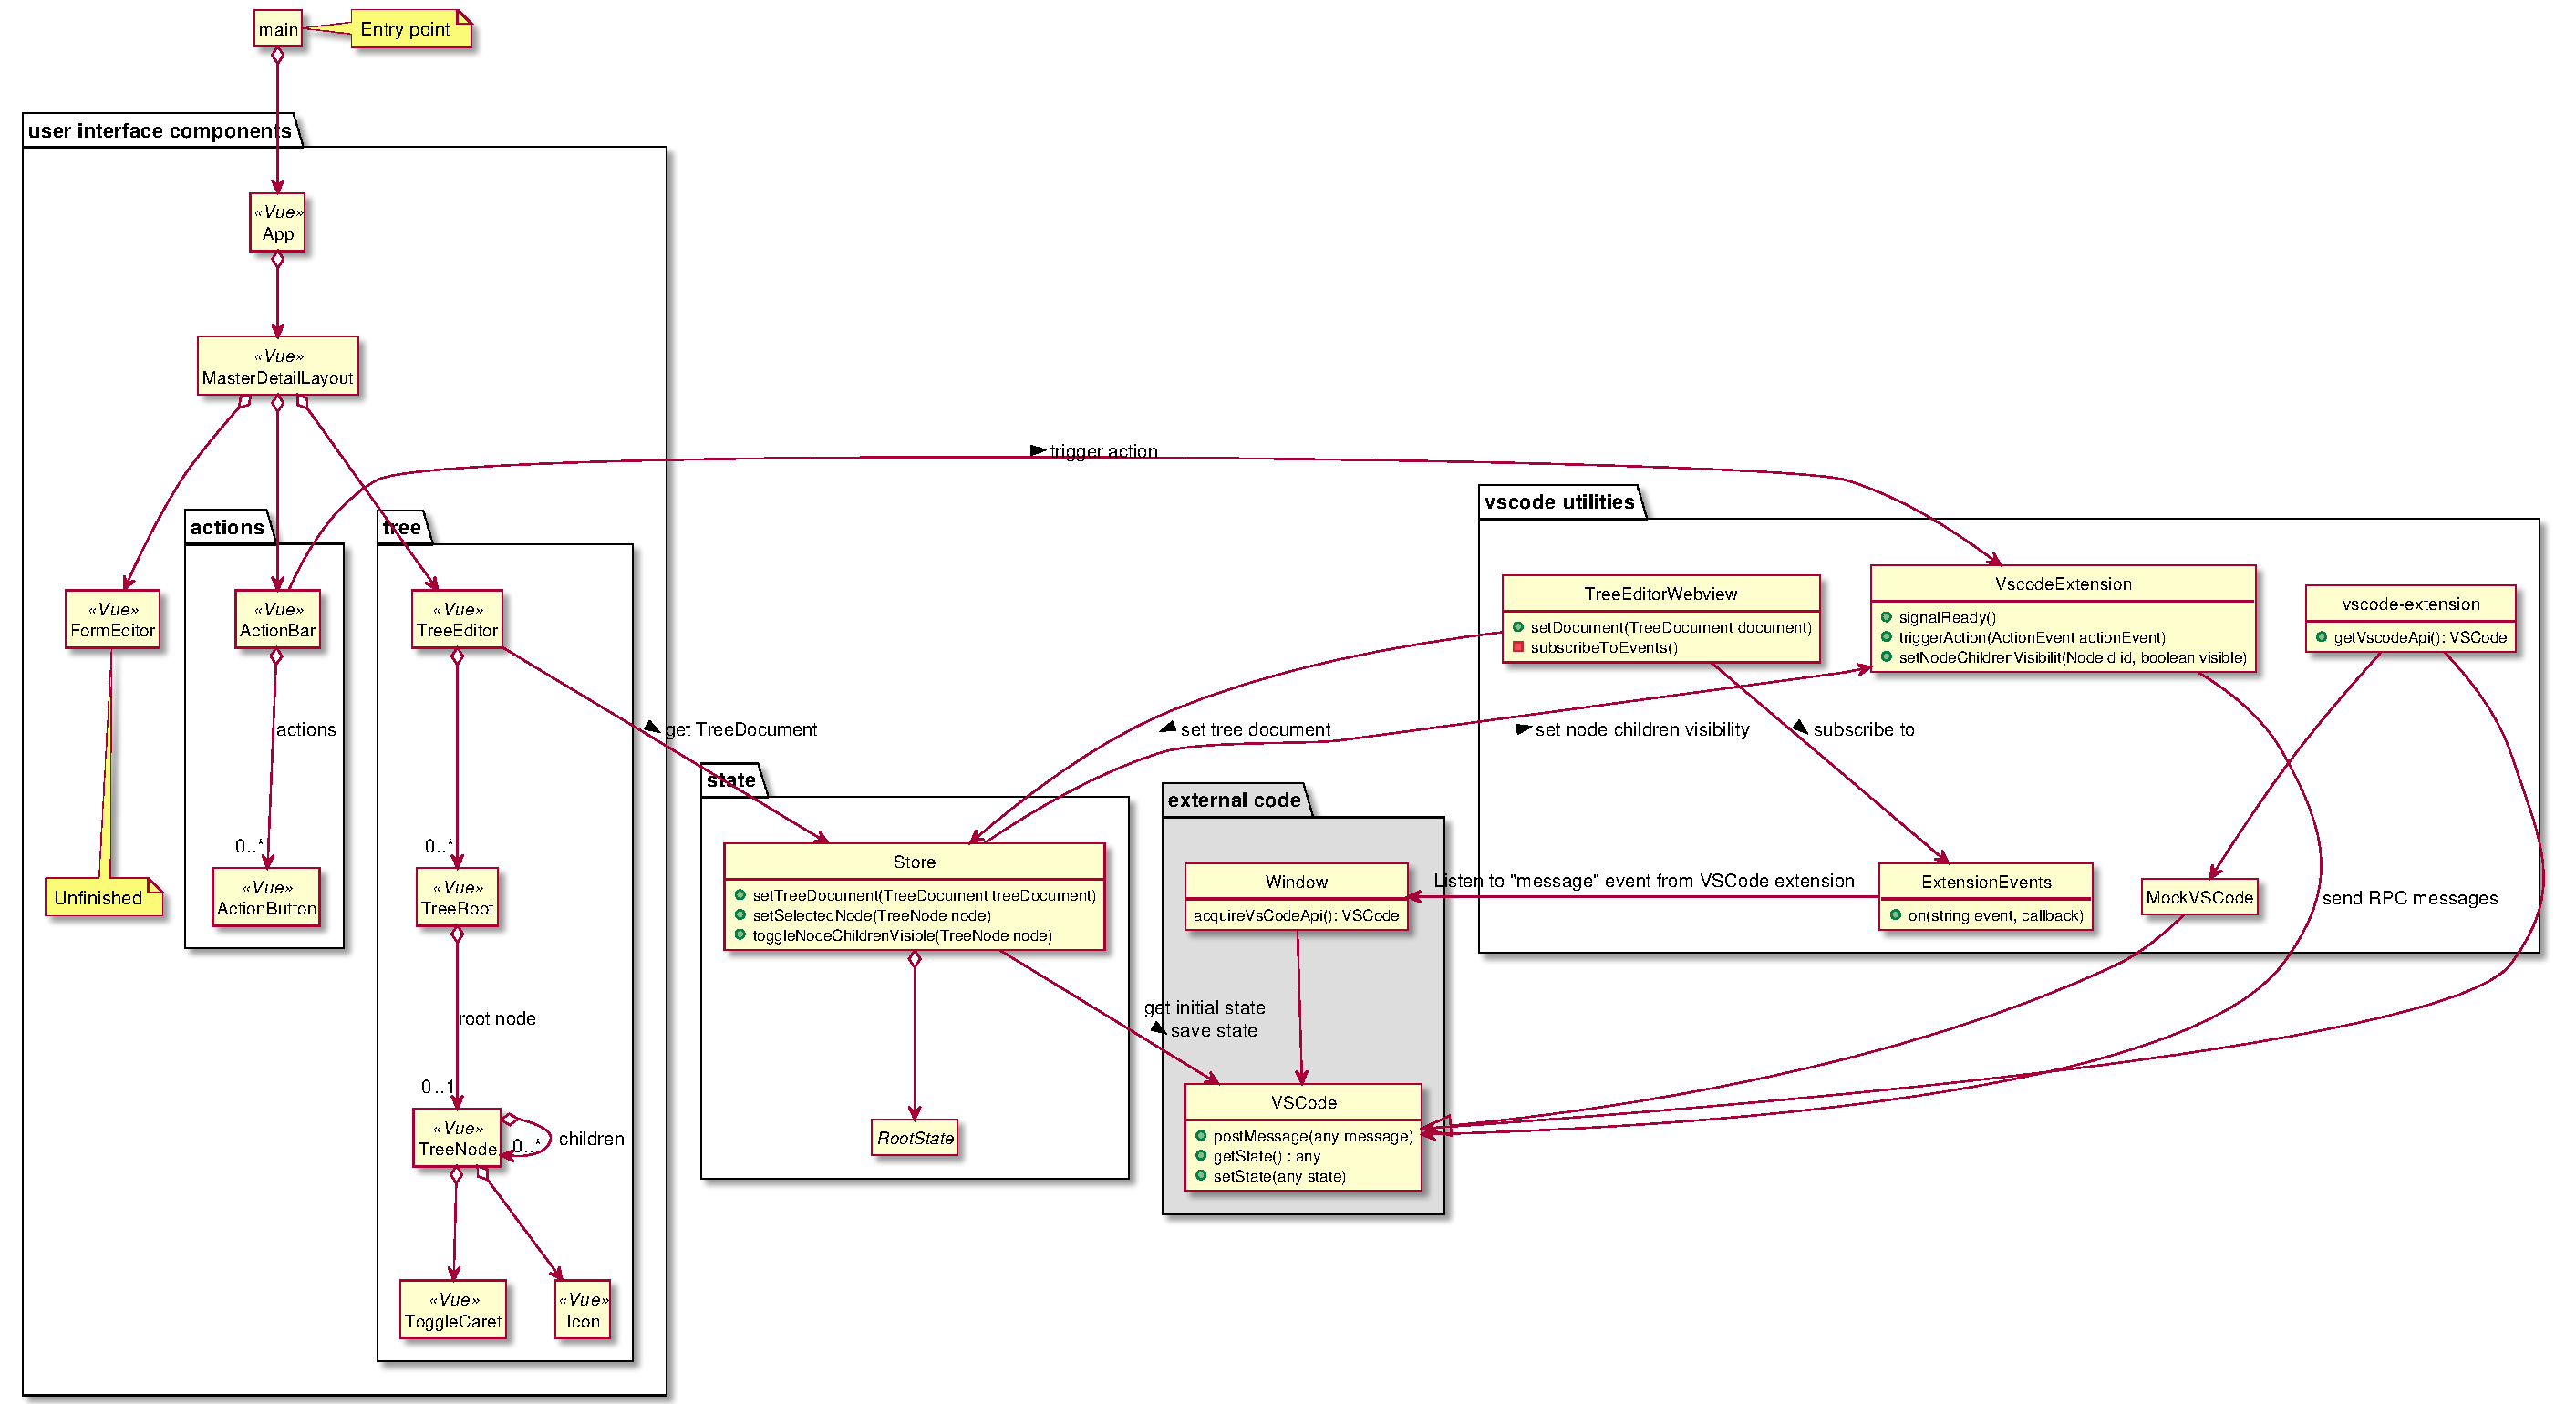
\includegraphics[width=\textwidth,height=1.2\textheight,keepaspectratio]{figures/plantuml/Tree_Editor_Frontend_code.pdf}
  \caption[Tree Editor Frontend class diagram]{Class diagram of the Tree Editor Frontend component.}\label{fig:tree-editor-frontend-code}
\end{sidewaysfigure}

\FloatBarrier

\paragraph{Extension classes}
A diagram of the \gls{VSCode} extension is shown in \cref{fig:tree-editor-extension-code}.
The execution environment for this is \gls{Nodejs}.
The \texttt{extension} file is activated by \gls{VSCode} when particular triggers specified in the extension's \texttt{package.json} manifest occur.
One such trigger is opening a \texttt{.ecore} file.
The \texttt{extension} then registers commands and the custom editor.
The \texttt{CustomTreeEditorProvider} is asked by \gls{VSCode} to create a document and editor for the \texttt{.ecore} file.
The editor uses the compiled outputs of the frontend, and puts it inside a \texttt{WebView}.
A \texttt{WebView} is an isolated execution context provided by \gls{VSCode} (analogous to an \texttt{IFrame} in HTML), where a custom user interface can be shown.
An extension is otherwise not allowed to modify the user interface in \gls{VSCode}.\\

The extension also starts a java process with the executable \texttt{.jar} file for the server.
It then attaches to the \textit{standard in} and \textit{standard out} as communication channels for the \acrshort{TLSP}.
The communication and protocol parsing uses the \texttt{vscode-jsonrpc} library from Microsoft, also used in the official \acrshort{LSP} implementation for \gls{VSCode}.

\begin{sidewaysfigure}[htbp]  % order of priority: h here, t top, b bottom, p page
  \centering
  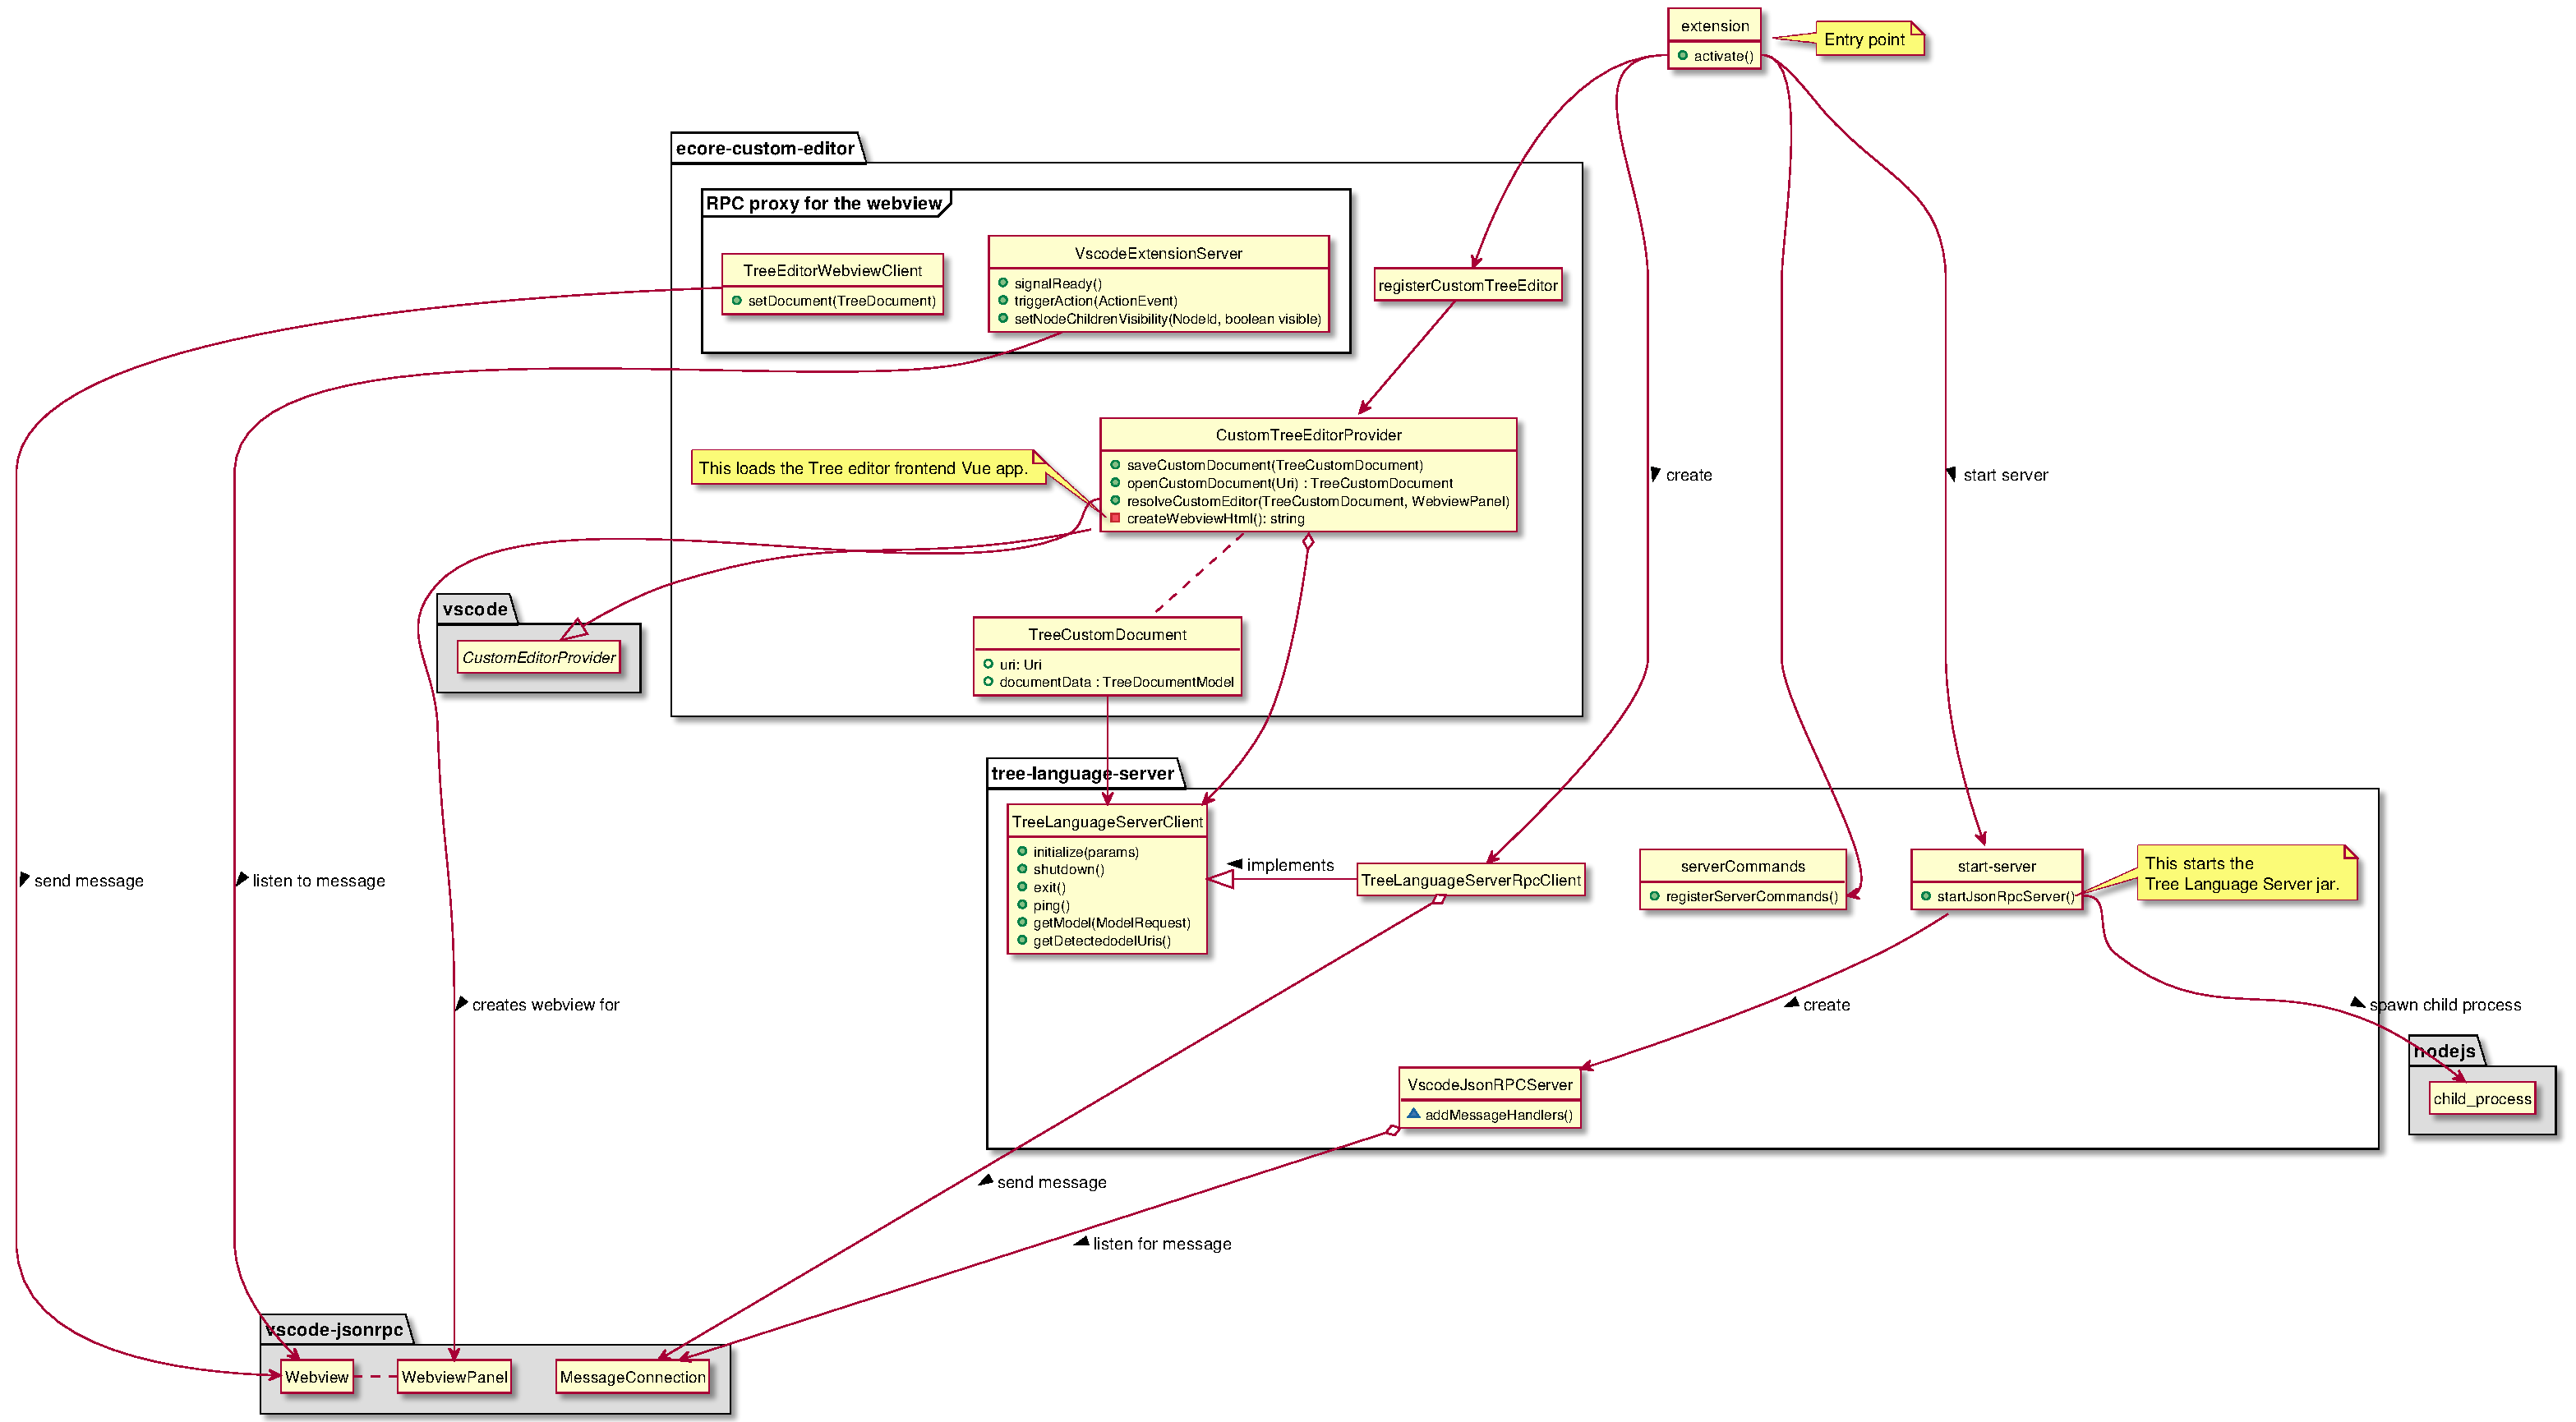
\includegraphics[width=\textwidth,height=1.2\textheight,keepaspectratio]{figures/plantuml/Tree_Editor_Extension_code.pdf}
  \caption[Tree Editor Extension class diagram]{Class diagram of the Tree Editor Extension component.}\label{fig:tree-editor-extension-code}
\end{sidewaysfigure}

\FloatBarrier

\paragraph{Server classes}
A diagram of the server is shown in \cref{fig:tree-editor-server-code}.
The \acrshort{TLSP} server for \acrshort{EMF} starts a \gls{JSON-RPC} server listening to \textit{standard in} and \textit{standard out}, to communicate with the extension.
The protocol is defined with two annotated java interfaces: \texttt{Server} and \texttt{Client}.
The \texttt{Server} represent this server itself, while the \texttt{Client} is the \gls{VSCode} extension side.
An implementation of the \texttt{Server} interface is central, as it does the actual logic in the \acrlong{TLSP}.
The \texttt{ServerImpl} and \texttt{Client} are handed to a \texttt{Launcher}, which comes from the \textit{LSP4J} project.
This is an Eclipse Foundation project which provides a Java \acrshort{LSP}.
Here, the \gls{JSON-RPC} component is standalone, and reused here, with the \acrshort{TLSP} as protocol instead of \acrshort{LSP}.\\

The \texttt{ServerImpl} delegates most of the work to an \texttt{EmfTreeModelController}, which in turn delegates to the EMF.Cloud Model Server or a \texttt{EcoreToTreeDocumentMapper}.
The latter uses the \acrshort{EMF} runtime \acrshort{API} and \texttt{ReflectiveItemProvider} from the \texttt{.edit} \acrshort{EMF} package.
The \texttt{EcoreToTreeDocumentMapper} maps a \acrshort{EMF} \texttt{Resource} to a \texttt{TreeDocument} data structure, compatible with the one in the Tree Document model library component for javascript.

\begin{sidewaysfigure}[htbp]  % order of priority: h here, t top, b bottom, p page
  \centering
  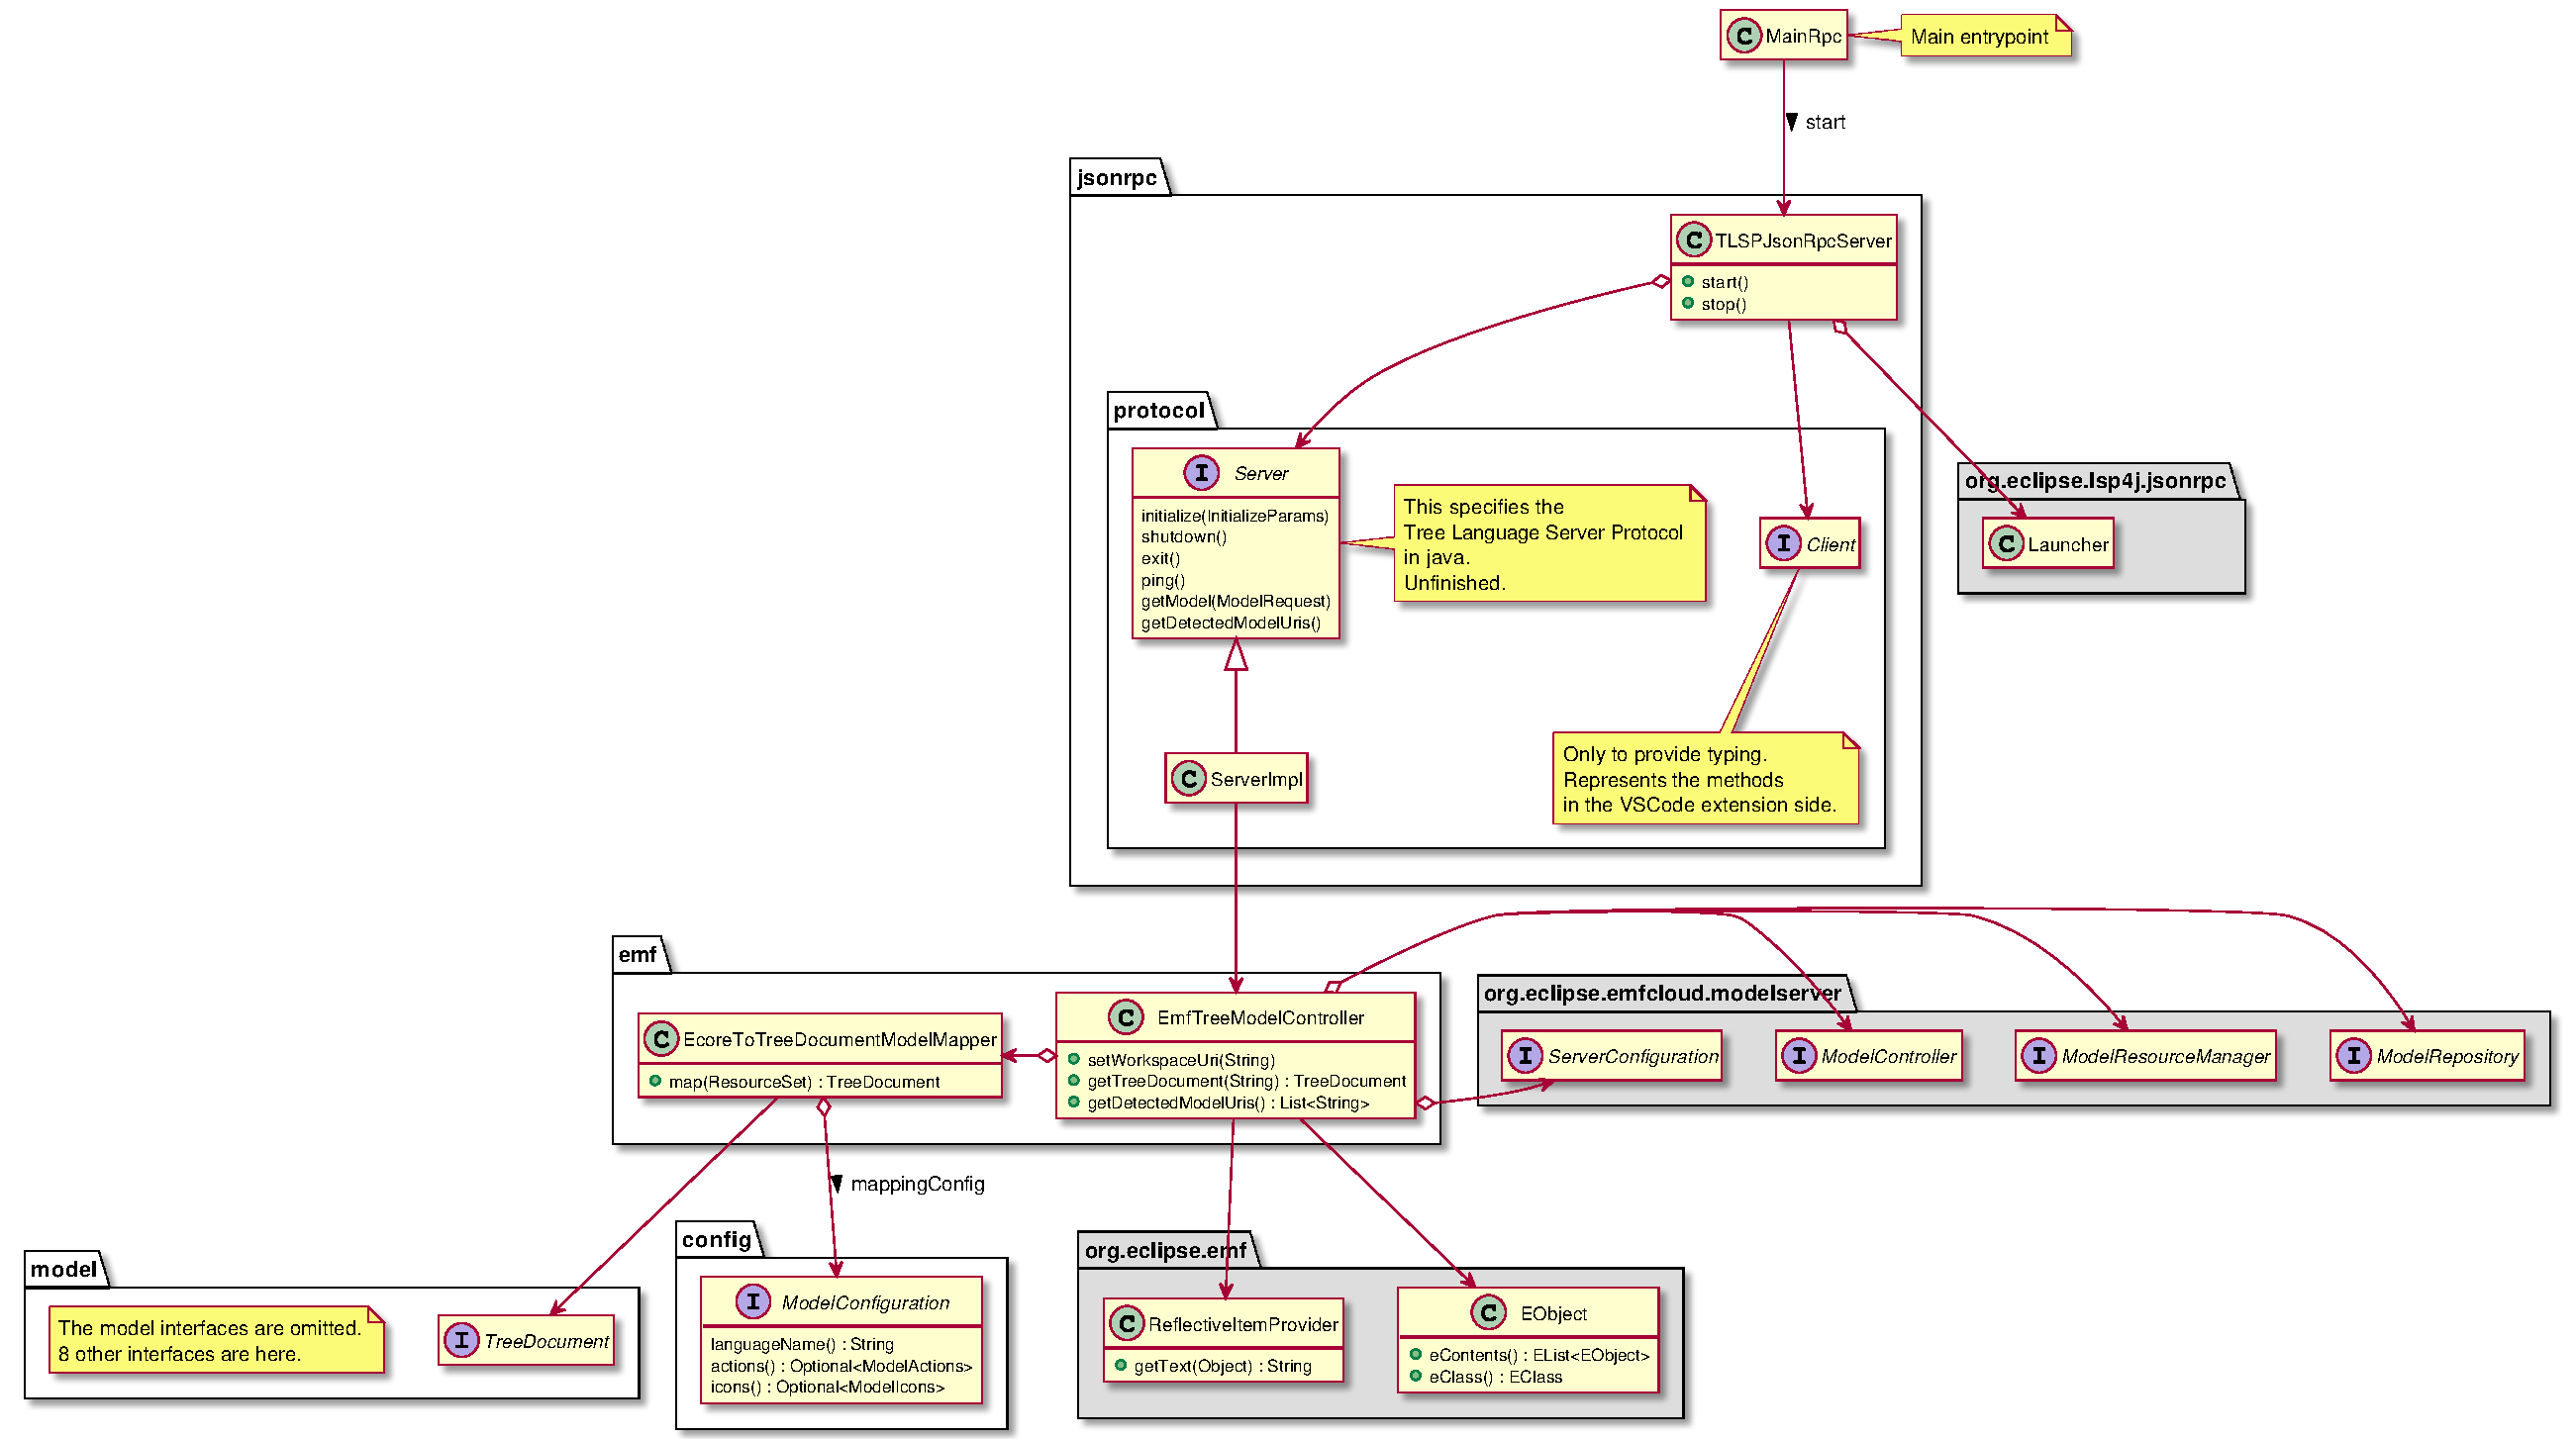
\includegraphics[width=\textwidth,height=\textheight,keepaspectratio]{figures/plantuml/Tree_Language_Server_code.pdf}
  \caption[Tree Language Server class diagram]{Class diagram of the Tree Language Server component.}\label{fig:tree-editor-server-code}
\end{sidewaysfigure}

\FloatBarrier
